\documentclass[fleqn,reqno,10pt,draft]{article}

\usepackage{myarticlestyledefault}


\usepackage{mypackages}
\usepackage{mycommands}
\usepackage{myenvironments}

\usepackage[]{svninfo}
\usepackage{subfig}



\newcommand{\lit}{\acro{lit}}
\newcommand{\glb}{\acro{glb}}
\newcommand{\loc}{\acro{loc}}

\newcommand{\as}{\acro{as}}
\renewcommand{\es}{\acro{es}}
\renewcommand{\AE}{\as}
\newcommand{\GE}{\es}

\newcommand{\lc}{\acro{lc}}
\newcommand{\ec}{\acro{ec}}
\newcommand{\LC}{\lc}
\newcommand{\EC}{\ec}


\DefineNamedColor{named}{mycol}{cmyk}{0.6,0.6,0,0}
\DefineNamedColor{named}{mygray}{cmyk}{0.05,0.05,0.05,0.05}
\DefineNamedColor{named}{mygraylight}{cmyk}{0.017,0.017,0.017,0.017}

\newcommand{\mymark}[1]{{\color{mycol}{#1}}}

\title{Scalar Items in Embedded Position: {A}nother Experimental Approach}
\author{Fabian Schlotterbeck, Michael Franke and Petra Augurzky}
\date{}

\begin{document}
\maketitle


\begin{abstract}
  \dots make concrete \dots
\end{abstract}

\svnInfo $Id$

\section{Introduction}
\label{sec:introduction}

This paper deals with the interpretation of two types of
sentences, namely:

\begin{exe}
\ex \label{bsp:AE}
  \mymark{All} of the students read \mymark{some} of the
  papers. \hfill (\AE)
\ex \label{bsp:GE} 
  \mymark{Exactly one} of the students read \mymark{some} of the
  papers. \hfill (\GE)
\end{exe}

\noindent In \as-sentences a scalar item \emph{some} takes scope under
a universal quantifier \emph{all}. In \es-sentences a scalar item
\emph{some} takes scope under a non-monotonic quantifier \emph{exactly
  one}. Scalar \emph{some} is usually assumed to receive a semantic
interpretation similar to logical $\exists$, so that the sentence
\emph{Some boys cried} is literally true in a situation where all
boys cried. But it is also known to invite upper-bounding inferences
in plain utterances:

\begin{exe}
  \ex \label{bsp:Plain-SI}
    \begin{xlist}
      \ex \label{bsp:Plain-SI-Target} Hans solved some of the problems.
      \ex \label{bsp:Plain-SI-Implicature} $\implicates$ Hans solved some but not all of the problems.
    \end{xlist}
\end{exe}

\noindent The classical explanation of this inference, following the
pioneering work of \citet{Grice1975:Logic-and-Conve}, has it that
(\ref{bsp:Plain-SI-Implicature}) is a pragmatic inference, a so-called
\emph{quantity implicature}, derived by an abductive inference as the
best explanation of why am informed, knowledgable and cooperative
speaker has uttered (\ref{bsp:Plain-SI-Target}) when she could also
have uttered the semantically stronger and relevant:\dn{redo labels of
  examples}

\begin{exe}
  \exr{bsp:Plain-SI}
    \begin{xlist}
      \exi{c.} \label{bsp:Plain-SI-Alternative} Hans solved all of the problems.
    \end{xlist}
\end{exe}

\noindent If this upper-bounding inference would occur often and
systematically enough, then it may well be that also embedded
occurrences of \emph{some} get enriched, in some fashion or other, to
contribute the enriched meaning \emph{some but not all} also under the
scope of other logical operators. Indeed, even
\citeauthor{Grice1975:Logic-and-Conve} envisaged this possibility when
he wrote: ``It may not be impossible for what starts life, so to
speak, as a conversational implicature to become conventionalized''
\citep[p.58]{Grice1975:Logic-and-Conve}. But then there are at least
three relevant candidate readings for \as- and \es-sentences: (i) a
\emph{literal reading} like in (\ref{bsp:AE-Literal}) and
(\ref{bsp:GE-Literal}) where \emph{some} has only its literal meaning;
(ii) a \emph{global reading} like in (\ref{bsp:AE-Global}) and
(\ref{bsp:GE-Global}) where, according to the Gricean intuition, we
enrich utterances of (\ref{bsp:AE}) and (\ref{bsp:GE}) with the
negation of alternativ utterances of the corresponding sentences
(\ref{bsp:AE-Alternative}) and (\ref{bsp:GE-Alternative}) where
\emph{some} is replaced by \emph{all}; and also (iii) a \emph{local
  reading} like in (\ref{bsp:AE-Local}) and (\ref{bsp:GE-Local}) where
\emph{some} is read to mean \emph{some but not all} in the scope of
the embedding quantifier.


% DIRTY!!!
\setcounter{exx}{0}

\begin{exe}

  \ex \mymark{All} of the students read {\mymark{some}} of the
  papers. 

  \begin{xlist}
  \ex \label{bsp:AE-Literal} \mymark{All} of the students read
    {\mymark{some and maybe all}} of the papers. \hfill (\as-\lit)
  \ex \label{bsp:AE-Global}
    \mymark{All} of the students read \mymark{some} 
    and  \hfill (\as-\glb)\\
    \mymark{not all} of the students read \mymark{all} of the papers.
  \ex \label{bsp:AE-Local}
    \mymark{All} of the students read {\mymark{some  but not all}} of the
    papers. \hfill (\as-\loc)
  \end{xlist}

\ex \mymark{Exactly one} of the students read {\mymark{some}} of the
  papers.

  \begin{xlist}
  \ex \label{bsp:GE-Literal} \mymark{Exactly one} of the students read
    {\mymark{some and maybe all}} of the papers. \hfill (\es-\lit)
  \ex \label{bsp:GE-Global}
    \mymark{Exactly one} of the students read \mymark{some} 
    and  \hfill (\es-\glb)\\
    \mymark{not all} of the students read \mymark{all} of the papers.
  \ex \label{bsp:GE-Local}
    \mymark{Exactly one} of the students read {\mymark{some  but not all}} of the
    papers. \hfill (\es-\loc)
  \end{xlist}

\ex \label{bsp:AE-Alternative} \mymark{All} of the students read
  {\mymark{all}} of the papers. 

\ex \label{bsp:GE-Alternative} \mymark{Exactly one} of the students
  read {\mymark{all}} of the papers.

\end{exe}

\noindent Section~\ref{sec:get-know-your} will discuss these reading
in more detail and, by giving some helpful illustrations, make clear
that these readings are all distinct but logically dependent
on each other in interesting ways.

The main question we are interested in here is which of these three
conceivable readings is available to subjects na\"{i}ve to all
pragmatic theory. We are moreover interested in the more refined
question which of the available readings na\"{i}ve subjects prefer.

Addressing these issues empirically is highly relevant because they
lie at the heart of the current debate of the exact location and
nature of the interface between semantics and pragmatics. There are
three major camps which are ---more or less fiercely--- involved in
this border war, all of which make different predictions about
availability and preferences of readings. We will give a more detailed
description of the various theoretical positions below in
Section~\ref{sec:theories-predictions}, but on a first rough
approximation the situation is the following. Firstly, there are
\mymark{pragmatic traditionalists} who seek to conserve the spirit of
\citeauthor{Grice1975:Logic-and-Conve}'s
(\citeyear{Grice1975:Logic-and-Conve}) original ideas as much as
possible
\citep[e.g.][]{Spector2006:Scalar-Implicat,Sauerland2004:Scalar-Implicat,Russell2006:Against-Grammat,vanRooijSchulz:ExhaustiveInterpretation,Geurts2010:Quantity-Implic,Franke2011:Quantity-Implic}. Traditionalists
happily acknowledge the existence of global readings, but might
consider local readings either unavailable or a beast distinct from
scalar implicatures. Opposed to that is the camp of \mymark{lexical
  conventionalists}
\citep[e.g.][]{LevinsonPresumptiveMeanings2000,Chierchia:2004_ScalarImplicatures}
who maintain that scalar \emph{some} is lexically ambiguous between
the standard logical meaning \emph{some and maybe all} and the
upper-bounded meaning \emph{some but not all}. As the latter is
considered a default, lexical conventionalism has no problem
accounting for local readings, and in fact would consider these the
preferred readings. Thirdly and finally, there is the camp of
\mymark{grammaticalists} who defend that the distribution of
upper-bounded readings of \emph{some} is best explained by postulating
a silent operator, akin to the meaning of the particle \emph{only}
\citep{Chierchia2006:Broaden-Your-Vi,Fox2007:Free-Choice-and,ChierchiaFox2008:The-Grammatical,Chierchia2012:FC-Nominals-and,Sauerland2012:The-Computation}. According
to the grammatical view, this silent operator may be applied in
compositional semantics also in the scope of other logical operators,
but the availability of readings is constraint by the \emph{strongest
  meaning hypothesis}
\citep{DalrympleKanazawa1998:Reciprocal-Expr}. Details follow in
Section~\ref{sec:theories-predictions}, but suffice it to just state
already that grammaticalist theories predict that all three types of
readings are available. Moreover, according to the grammatical view,
the local reading is preferred for \as-sentences, while the global one
is preferred for \es-sentences. (More precisely, as we will see
Section~\ref{sec:theories-predictions}, depending on the variant of
the strongest meaning hypothesis employed, either the global reading
is predicted to be preferred for \es-sentences, or the global and the
local reading are predicted to be equally preferred.)

Due to its theoretical significance, a number of previous studies have
already probed into the availability of readings for \as- and
\es-sentences
\citep[e.g.][]{GeurtsPouscoulous2009:Embedded-Implic,CliftonDube2010:Embedded-Implic,ChemlaSpector2010:Experimental-Ev}. However,
as we will argue in Section~\ref{sec:previous-studies}, results have
not been as clear-cut as one might have hoped for. Even worse so,
taken in conjunction, the empirical evidence is inconclusive as to
whether local readings exist. We hypothesized that previous studies
might be insufficiently informative because of the focus on (variants
of) a picture-verification paradigm.\dn{relate to Bob van Tiel's
  work}.  The problem is that in order to test the availability of
different candidate meanings different pictures have to be presented,
so that effects of pictorial complexity or stereotypicality could
never be ruled out entirely. Moreover, previous studies have only
accumulated limited evidence pertaining to the second question that
may help decide between theoretical positions, namely which of the
attested readings subjects prefer.

In reaction to this situation, we therefore studied a different mode
of visual presentation: subjects were presented with pictures that
were partly covered and could incrementally be uncovered at the
subjects' request; for each ((partially) covered) picture, subjects
had to decide whether they could already give a truth-value judgement
or needed more information.\dn{mention who else does this} This way we
obtained behavioral data that is both indicative of the reading
subjects assumed and independent of the complexity of the visual
stimulus. At the same time, we hypothesized that the incremental
nature of this task would shed light on the preferences over readings,
because the temporal distribution of truth-value judgments would give
away which reading subjects were waiting to evaluate, so to speak. To
test whether our method is indeed suitable to detect interpretation
preferences, we included ambiguous test items like
(\ref{bsp:target-related-filler}) which are known to preferentially
receive the late-closure reading in
(\ref{bsp:target-related-filler-LC}) and not the dispreferred, but
attested early-closure reading
(\ref{bsp:target-related-filler-EC}).\dn{insert references to
  literature on EC-LC processing}

\begin{exe}
\ex \label{bsp:target-related-filler} The letter is connected with circles and squares with
  suns.
  \begin{xlist}
  \ex \label{bsp:target-related-filler-LC} The letter is connected with circles and squares; the latter
    but not the former contain suns. \hfill (\LC)
  \ex \label{bsp:target-related-filler-EC} The letter is connected with circles and squares; both
    contain suns. \hfill (\EC)
  \end{xlist}
\end{exe}

\noindent Finally, since it is often argued (see
Section~\ref{sec:theories-predictions}) that intonational stress on an
embedded scalar item can favor a local reading we presented sentence
auditorily and manipulated stress accordingly. The design of our
studies is detailed in Section XYZ.

\begin{itemize}
\item summarize results
\end{itemize}

\section{Get to know your readings}
\label{sec:get-know-your}

\begin{figure}[]
  \centering
  
\subfloat[fig:false][false]{
  \label{fig:false}
  
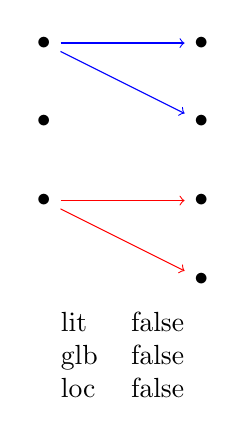
\begin{tikzpicture}[node distance = 1cm]
        % Nodes

        \node (X-1) {$\Large{\bullet}$};

        \node (X-2) [below of = X-1] {$\Large{\bullet}$};

        \node (X-3) [below of = X-2] {$\Large{\bullet}$};

        \node (Y-1) [right of = X-1, node distance = 2cm]{$\Large{\bullet}$};

        \node (Y-2) [below of = Y-1] {$\Large{\bullet}$};

        \node (Y-3) [below of = Y-2] {$\Large{\bullet}$};

        \node (Y-4) [below of = Y-3] {$\Large{\bullet}$};

        % table added from here

        \node (X-4) [below of = X-3, node distance = 2cm] {};

        \node (table) [right of = X-4] {
          \begin{tabular}{ll}
            \lit & false \\
            \glb & false \\
            \loc & false 
          \end{tabular}};

        % Arrows

        \path [draw=blue,->] (X-1) -> (Y-1);

        \path [draw=blue,->] (X-1) -> (Y-2);


        \path [draw=red,->] (X-3) -> (Y-3);

        \path [draw=red,->] (X-3) -> (Y-4);

      \end{tikzpicture}

}
\subfloat[fig:literal][literal]{
  \label{fig:literal}

  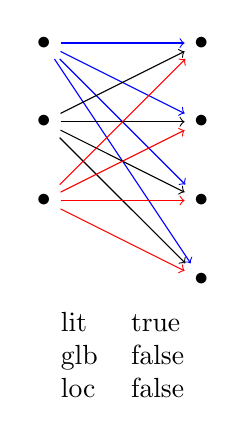
\begin{tikzpicture}[node distance = 1cm]
        % Nodes

        \node (X-1) {$\Large{\bullet}$};

        \node (X-2) [below of = X-1] {$\Large{\bullet}$};

        \node (X-3) [below of = X-2] {$\Large{\bullet}$};

        \node (Y-1) [right of = X-1, node distance = 2cm]{$\Large{\bullet}$};

        \node (Y-2) [below of = Y-1] {$\Large{\bullet}$};

        \node (Y-3) [below of = Y-2] {$\Large{\bullet}$};

        \node (Y-4) [below of = Y-3] {$\Large{\bullet}$};

        % table added from here

        \node (X-4) [below of = X-3, node distance = 2cm] {};

        \node (table) [right of = X-4] {
          \begin{tabular}{ll}
            \lit & true \\
            \glb & false \\
            \loc & false 
          \end{tabular}};

        % Arrows

        \path [draw=blue,->] (X-1) -> (Y-1);

        \path [draw=blue,->] (X-1) -> (Y-2);

        \path [draw=blue,->] (X-1) -> (Y-3);

        \path [draw=blue,->] (X-1) -> (Y-4);


        \path [draw=black,->] (X-2) -> (Y-1);

        \path [draw=black,->] (X-2) -> (Y-2);

        \path [draw=black,->] (X-2) -> (Y-3);

        \path [draw=black,->] (X-2) -> (Y-4);



        \path [draw=red,->] (X-3) -> (Y-1);

        \path [draw=red,->] (X-3) -> (Y-2);

        \path [draw=red,->] (X-3) -> (Y-3);

        \path [draw=red,->] (X-3) -> (Y-4);

      \end{tikzpicture}

}
\subfloat[fig:weak][weak]{
  \label{fig:weak}

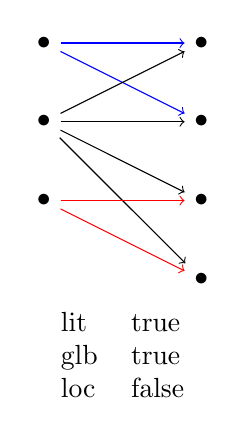
\begin{tikzpicture}[node distance = 1cm]
        % Nodes

        \node (X-1) {$\Large{\bullet}$};

        \node (X-2) [below of = X-1] {$\Large{\bullet}$};

        \node (X-3) [below of = X-2] {$\Large{\bullet}$};

        \node (Y-1) [right of = X-1, node distance = 2cm]{$\Large{\bullet}$};

        \node (Y-2) [below of = Y-1] {$\Large{\bullet}$};

        \node (Y-3) [below of = Y-2] {$\Large{\bullet}$};

        \node (Y-4) [below of = Y-3] {$\Large{\bullet}$};

        % table added from here

        \node (X-4) [below of = X-3, node distance = 2cm] {};

        \node (table) [right of = X-4] {
          \begin{tabular}{ll}
            \lit & true \\
            \glb & true \\
            \loc & false 
          \end{tabular}};

        % Arrows

        \path [draw=blue,->] (X-1) -> (Y-1);

        \path [draw=blue,->] (X-1) -> (Y-2);


        \path [draw=black,->] (X-2) -> (Y-1);

        \path [draw=black,->] (X-2) -> (Y-2);

        \path [draw=black,->] (X-2) -> (Y-3);

        \path [draw=black,->] (X-2) -> (Y-4);


        \path [draw=red,->] (X-3) -> (Y-3);

        \path [draw=red,->] (X-3) -> (Y-4);

      \end{tikzpicture}


}
\subfloat[fig:strong][strong]{
  \label{fig:strong}

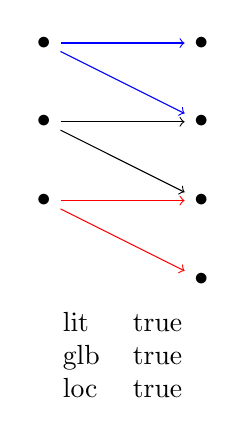
\begin{tikzpicture}[node distance = 1cm]
        % Nodes

        \node (X-1) {$\Large{\bullet}$};

        \node (X-2) [below of = X-1] {$\Large{\bullet}$};

        \node (X-3) [below of = X-2] {$\Large{\bullet}$};

        \node (Y-1) [right of = X-1, node distance = 2cm]{$\Large{\bullet}$};

        \node (Y-2) [below of = Y-1] {$\Large{\bullet}$};

        \node (Y-3) [below of = Y-2] {$\Large{\bullet}$};

        \node (Y-4) [below of = Y-3] {$\Large{\bullet}$};

        % table added from here

        \node (X-4) [below of = X-3, node distance = 2cm] {};

        \node (table) [right of = X-4] {
          \begin{tabular}{ll}
            \lit & true \\
            \glb & true \\
            \loc & true 
          \end{tabular}};

        % Arrows

        \path [draw=blue,->] (X-1) -> (Y-1);

        \path [draw=blue,->] (X-1) -> (Y-2);


        \path [draw=black,->] (X-2) -> (Y-2);

        \path [draw=black,->] (X-2) -> (Y-3);


        \path [draw=red,->] (X-3) -> (Y-3);

        \path [draw=red,->] (X-3) -> (Y-4);

      \end{tikzpicture}



}

  

  \caption{Distinguishing scenarious for \as-sentences}
  \label{fig:AS-distinguishing-pics}
\end{figure}


\begin{figure}[]
  \centering
  
\subfloat[fig:false][false]{
  \label{fig:false}

  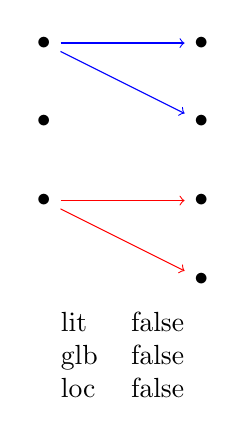
\begin{tikzpicture}[node distance = 1cm]
        % Nodes

        \node (X-1) {$\Large{\bullet}$};

        \node (X-2) [below of = X-1] {$\Large{\bullet}$};

        \node (X-3) [below of = X-2] {$\Large{\bullet}$};

        \node (Y-1) [right of = X-1, node distance = 2cm]{$\Large{\bullet}$};

        \node (Y-2) [below of = Y-1] {$\Large{\bullet}$};

        \node (Y-3) [below of = Y-2] {$\Large{\bullet}$};

        \node (Y-4) [below of = Y-3] {$\Large{\bullet}$};

        % table added from here

        \node (X-4) [below of = X-3, node distance = 2cm] {};

        \node (table) [right of = X-4] {
          \begin{tabular}{ll}
            \lit & false \\
            \glb & false \\
            \loc & false 
          \end{tabular}};


        % Arrows

        \path [draw=blue,->] (X-1) -> (Y-1);

        \path [draw=blue,->] (X-1) -> (Y-2);


        \path [draw=red,->] (X-3) -> (Y-3);

        \path [draw=red,->] (X-3) -> (Y-4);

      \end{tikzpicture}


}
\subfloat[fig:literal][literal]{
  \label{fig:literal}

      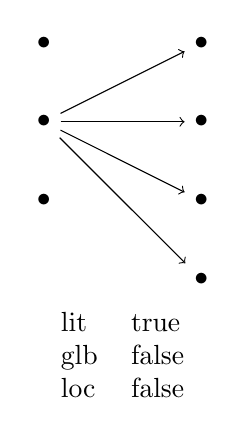
\begin{tikzpicture}[node distance = 1cm]
        % Nodes

        \node (X-1) {$\Large{\bullet}$};

        \node (X-2) [below of = X-1] {$\Large{\bullet}$};

        \node (X-3) [below of = X-2] {$\Large{\bullet}$};

        \node (Y-1) [right of = X-1, node distance = 2cm]{$\Large{\bullet}$};

        \node (Y-2) [below of = Y-1] {$\Large{\bullet}$};

        \node (Y-3) [below of = Y-2] {$\Large{\bullet}$};

        \node (Y-4) [below of = Y-3] {$\Large{\bullet}$};

        % table added from here

        \node (X-4) [below of = X-3, node distance = 2cm] {};

        \node (table) [right of = X-4] {
          \begin{tabular}{ll}
            \lit & true \\
            \glb & false \\
            \loc & false 
          \end{tabular}};

        % Arrows

        \path [draw=black,->] (X-2) -> (Y-1);

        \path [draw=black,->] (X-2) -> (Y-2);

        \path [draw=black,->] (X-2) -> (Y-3);

        \path [draw=black,->] (X-2) -> (Y-4);

      \end{tikzpicture}

}
\subfloat[fig:local][local]{
  \label{fig:local}

            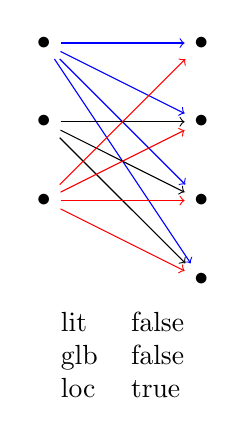
\begin{tikzpicture}[node distance = 1cm]
        % Nodes

        \node (X-1) {$\Large{\bullet}$};

        \node (X-2) [below of = X-1] {$\Large{\bullet}$};

        \node (X-3) [below of = X-2] {$\Large{\bullet}$};

        \node (Y-1) [right of = X-1, node distance = 2cm]{$\Large{\bullet}$};

        \node (Y-2) [below of = Y-1] {$\Large{\bullet}$};

        \node (Y-3) [below of = Y-2] {$\Large{\bullet}$};

        \node (Y-4) [below of = Y-3] {$\Large{\bullet}$};

        % table added from here

        \node (X-4) [below of = X-3, node distance = 2cm] {};

        \node (table) [right of = X-4] {
          \begin{tabular}{ll}
            \lit & false \\
            \glb & false \\
            \loc & true 
          \end{tabular}};

        % Arrows

        \path [draw=blue,->] (X-1) -> (Y-1);

        \path [draw=blue,->] (X-1) -> (Y-2);

        \path [draw=blue,->] (X-1) -> (Y-3);

        \path [draw=blue,->] (X-1) -> (Y-4);



        \path [draw=black,->] (X-2) -> (Y-2);

        \path [draw=black,->] (X-2) -> (Y-3);

        \path [draw=black,->] (X-2) -> (Y-4);



        \path [draw=red,->] (X-3) -> (Y-1);

        \path [draw=red,->] (X-3) -> (Y-2);

        \path [draw=red,->] (X-3) -> (Y-3);

        \path [draw=red,->] (X-3) -> (Y-4);

      \end{tikzpicture}

}
\subfloat[fig:all][all]{
  \label{fig:all}

      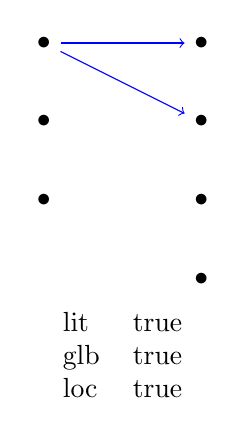
\begin{tikzpicture}[node distance = 1cm]
        % Nodes

        \node (X-1) {$\Large{\bullet}$};

        \node (X-2) [below of = X-1] {$\Large{\bullet}$};

        \node (X-3) [below of = X-2] {$\Large{\bullet}$};

        \node (Y-1) [right of = X-1, node distance = 2cm]{$\Large{\bullet}$};

        \node (Y-2) [below of = Y-1] {$\Large{\bullet}$};

        \node (Y-3) [below of = Y-2] {$\Large{\bullet}$};

        \node (Y-4) [below of = Y-3] {$\Large{\bullet}$};

        % table added from here

        \node (X-4) [below of = X-3, node distance = 2cm] {};

        \node (table) [right of = X-4] {
          \begin{tabular}{ll}
            \lit & true \\
            \glb & true \\
            \loc & true 
          \end{tabular}};

        % Arrows

        \path [draw=blue,->] (X-1) -> (Y-1);

        \path [draw=blue,->] (X-1) -> (Y-2);

      \end{tikzpicture}

}

  \caption{Distinguishing scenarious for \es-sentences}
  \label{fig:ES-distinguishing-pics}

\end{figure}


\section{Theories and predictions}
\label{sec:theories-predictions}

\section{Previous studies}
\label{sec:previous-studies}





\printbibliography[heading=bibintoc]

\end{document}
